\documentclass[tikz]{standalone}
\usepackage{tikz}
\usepackage{fourier-otf}
\usepackage{fontspec}

\usetikzlibrary{calc}

\begin{document}
	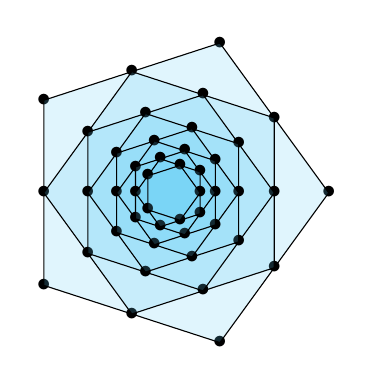
\begin{tikzpicture}
		\coordinate (A) at (0:2);
		\coordinate (B) at (72:2);
		\coordinate (C) at (2*72:2);
		\coordinate (D) at (3*72:2);
		\coordinate (E) at (4*72:2);
		\coordinate (F) at (A);
		\foreach \i in {0,...,8} {
			\draw(A) node {$\bullet$};
			\draw(B) node {$\bullet$};
			\draw(C) node {$\bullet$};
			\draw(D) node {$\bullet$};
			\draw(E) node {$\bullet$};
			
			\draw[fill=cyan!60, fill opacity=0.2](A) -- (B) -- (C) -- (D) -- (E) -- (A);
			
			\coordinate (A) at ($(A)!0.5!(B)$);
			\coordinate (B) at ($(B)!0.5!(C)$);
			\coordinate (C) at ($(C)!0.5!(D)$);
			\coordinate (D) at ($(D)!0.5!(E)$);
			\coordinate (E) at ($(E)!0.5!(F)$);
			\coordinate (F) at (A);
		}
	\end{tikzpicture}
\end{document}